\documentclass[a4paper, 11pt]{book}
\usepackage{/home/nicolas/Documents/Enseignement/Prepa/bpep/fichiers_utiles/preambule}
\newcommand{\qed}{\tag*{$\blacksquare$}}

\newcommand{\dsNB}{20}
\makeatletter
\renewcommand{\@chapapp}{Kh\^olles MPSI3 -- semaine \dsNB}
\makeatother

\toggletrue{corrige}  % décommenter pour passer en mode corrigé

% IMPORTS automatiques
\newcommand{\f}[2]{{
		\mathchoice
		{\dfrac{#1}{#2}}
		{\dfrac{#1}{#2}}
		{\frac{#1}{#2}}
		{\frac{#1}{#2}}
}}

\newcommand{\e}[1]{{}_{\text{#1}}}
\renewcommand{\a}[0]{\alpha}
\newcommand{\w}[0]{\omega}

\usepackage{physics}

 % fin des IMPORTS automatiques

\begin{document}

\chapter{Sujet 1\siCorrige{\!\!-- corrig\'e}}
\section{Question de cours}

Définir le moment cinétique d'un point matériel par rapport à un point et à un
axe, et le moment d'une force par rapport à un point et à un axe. Expliquer ce
qu'est le bras de levier \textbf{avec un schéma}, et énoncer le lien entre
moment d'une force et bras de levier. Démonstration \textbf{pour $\vv{F} \perp$
à l'axe}.

\resetQ
\subimport{/home/nicolas/Documents/Enseignement/Prepa/bpep/exercices/Colle/etain/}{sujet.tex}

\chapter{Sujet 2\siCorrige{\!\!-- corrig\'e}}
\section{Question de cours}

En utilisant la constante des aires, déterminer l'expression de l'énergie
potentielle effective pour un mouvement à force centrale conservative. Donner
$\Ec_p$ pour un champ de force newtonien,  représenter $\Ec_{p,\rm eff}$ et
discuter de la nature du mouvement en fonction de l'énergie mécanique totale
(cas attractif \textbf{et} répulsif).

\resetQ
\section{Températures d'ébullition}
Les températures d'ébullition sous \SI{1}{bar} des composés hydrogénés de la
14\ieme\ colonne et de la 17\ieme\ colonne du tableau périodique sont indiquées
sur le graphique ci-dessous~:

\begin{figure}[]
    \centering
    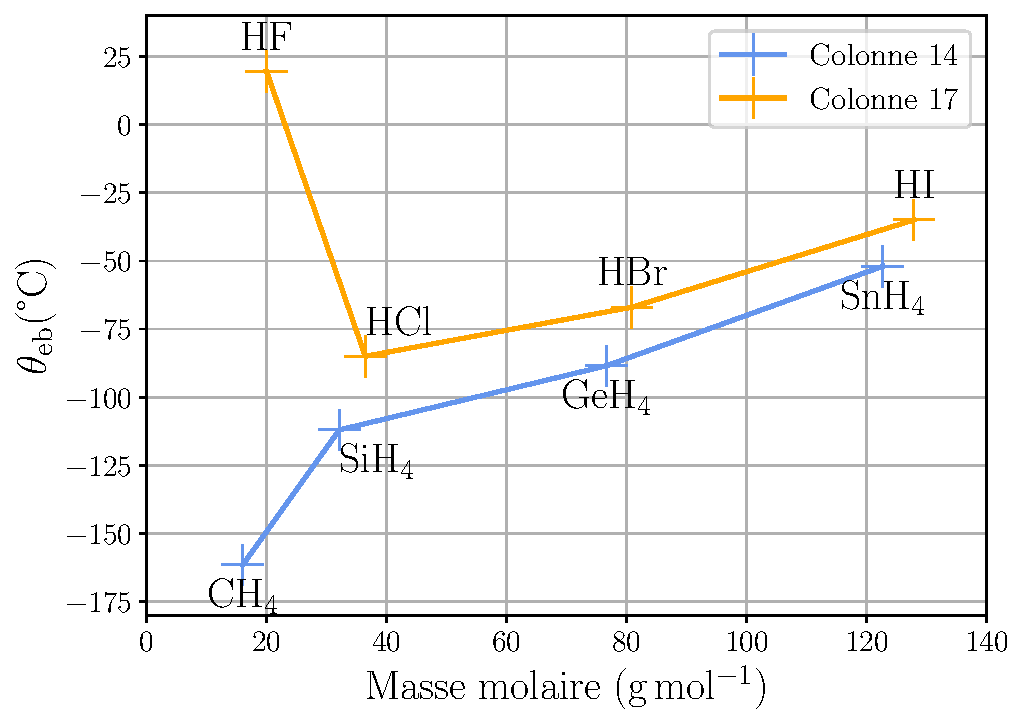
\includegraphics[scale=1]{../../figures/ch20/teb_hydro}
    \label{fig:tebhydro}
\end{figure}

\QR{La représentation de \textsc{Cram} de la molécule de méthane est
    représentée ci-dessous~:
    \begin{center}
        \chemfig{C(-[2]H)(<:[5]H)(<[6]H)(-[7]H)}
    \end{center}
    \begin{enumerate}
        \item En déduire le moment dipolaire de la molécule de méthane.
        \item En déduire la géométrie et le moment dipolaire des autres
            composés hydrogénés de la colonne 14.
    \end{enumerate}
}{
    \begin{enumerate}
        \item Par symétrie, la molécule de méthane ne possède pas de moment
            dipolaire permanent (les moments des quatre liaisons \ce{C-H} se
            compensent).
        \item Tous les éléments d'une même colonne ont le même nombre
            d'électrons de valence. Par conséquent, leurs composés
            hydrogénés ont tous la même structure, et en particulier leur
            géométrie est la même que celle de la molécule de méthane en ne
            changeant que l'atome central. De même, tous les composés
            hydrogénés de la colonne du carbone n'ont pas de moment
            dipolaire permanent.
    \end{enumerate}

}
\QR{Pourquoi les composés hydrogénés des éléments de la colonne 14 ont-ils
    des température d'ébullition plus basses que celles des composés
    hydrogénés de la colonne 17~?
}{Les éléments de la famille des halogènes sont bien plus
    électronégatifs que l'hydrogène et les molécules ne sont pas
    symétriques. Tous les composés de type \ce{H-X} où \ce{X} est un
    halogène sont donc polaires. Ainsi les forces de \textsc{Van der Waals}
    entre les composés hydrogénés de la colonne 17 sont plus importantes
    qu'entre les composés hydrogénés de la colonne 14. Ce qui explique les
    différences de température d'ébullition.
}
\QR{Expliquer l'augmentation observée entre \ce{HCl} et \ce{HI}.
}{La masse molaire de \ce{HI} est plus élevée que celle de \ce{HCl}, ce
    qui indique que la molécule est davantage polarisable. Les interactions
    de \textsc{Van der Waals} entre molécules sont donc plus fortes dans le
    cas de l'iode que dans le cas du chlore, ce qui explique la croissance
    observée.
}
\QR{Proposer une explication à l'anomalie observée pour \ce{HF}.
}{L'atome de fluor appartient à la deuxième période et il est fortement
    électronégatif. Des liaisons hydrogène peuvent donc se former entre
    molécules de \ce{HF}, ce qui n'est pas possible dans les autres espèces
    chimiques. Comme ces liaisons sont beaucoup plus fortes que les autres
    interactions faibles, elles expliquent la forte anomalie de température
    d'ébullition observée pour \ce{HF}.
}

\chapter{Sujet 3\siCorrige{\!\!-- corrig\'e}}
\section{Question de cours}

Énoncer et démontrer le théorème du moment cinétique par rapport à un point et à
un axe~; application au pendule simple pour retrouver l'équation du mouvement.

\resetQ
\subimport{/home/nicolas/Documents/Enseignement/Prepa/bpep/exercices/Colle/halogenes/}{sujet.tex}

\chapter{Sujet 4\siCorrige{\!\!-- corrig\'e}}
\resetQ
\subimport{/home/nicolas/Documents/Enseignement/Prepa/bpep/exercices/TD/molecules_polaires/}{sujet.tex}

\section{Schémas de \textsc{Lewis}}
\resetQ
\begin{enumerate}
    \item Donner le schéma de \textsc{Lewis} des espèces suivantes~:
        \[
            \ce{CH2Cl2}
            \qquad
            \ce{O2}
            \qquad
            \ce{C2H4}
            \qquad
            \ce{H3O+}
            \qquad
            \ce{HO-}
            \qquad
            \ce{H2CO}
            \qquad
            \ce{SiO2}
            \qquad
            \ce{CH3NH2}
        \]
    \item L'ozone \ce{O3} est une molécule non cyclique. Proposer une structure.
    \item \textit{Formule de \textsc{Lewis} de l'acide sulfurique}
    \begin{enumerate}[]
        \item Donner le schéma de \textsc{Lewis} de l'acide sulfurique
            \ce{H2SO4}. Dans cette molécule, les quatre atomes d'oxygène sont
            reliés à l'atome de soufre.
        \item En déduire celles des ions \ce{HSO4-} et \ce{SO4^{2-}}.
    \end{enumerate}
    \item Donner le schéma de \textsc{Lewis} des ions hydrogénocarbonate
        \ce{HCO3-} et carbonate \ce{CO3^{2-}}.
    \item Donner le schéma de \textsc{Lewis} du benzène \ce{C6H6}, qui est une
        molécule cyclique.
\end{enumerate}
\label{LastPage}
\end{document}
